\section{Theorie}
\label{sec:Theorie}

\subsection{Interferenz und Kohärenz von Licht}
Licht wird in diesem Versuch als elektromagnetische Welle betrachtet, um Interferenzerscheinungen erklären zu können. Die elektrische Feldstärke ist 
ebenfalls eine solche Welle und kann über 
\begin{equation*}
    \vec{E} = \vec{E}_0\cos{kx-\omega t - \delta}
\end{equation*}
beschrieben werden. Die Ausbreitung von Licht wird dabei über die Maxwellschen Gleichungen beschrieben. Außerdem folgt das elektrische Feld 
$\vec{E}$ dem Prinzip der linearen Superposition.
Die Intensität berechnet sich durch 
\begin{equation*}
    I = \text{const.}\cdot \rvert\vec{E}\lvert^2 \; .
\end{equation*}
Bei einer Überlagerung von zwei Wellen ergibt sich für die Intensität 
\begin{equation*}
    I = 2\cdot \text{const.}\cdot \vec{E}_0^2 \cos{\delta_2-\delta_1} \; .
\end{equation*}
Wenn die Bedingung
\begin{equation*}
    \delta_2 -\delta_1 = \left(2n+1\right)\pi 
\end{equation*}
erfüllt ist, ergibt sich die Intensität zu null.

Bei zwei unabhängigen Lichtquellen, sind die Phasenkonstanten $\delta_1$ und $\delta_2$ statistische Funktionen der Zeit, wodurch es keine 
Interferenzerscheinung gibt. Dieses Licht ist dann inkohärent. Mithilfe eines LASERs (light amplification by stimulated emission of radiation)
ist es jedoch möglich kohärentes Licht zu erzeugen, welches ein festes $k$, $\omega$ und $\delta$ besitzt.
Bei einem Wegunterschied der einzelnen Strecken des Interferometers, der der Kohärenzlänge $l$ oder mehr entspricht, verschwindet jedoch die 
Interferenzerscheinung. Die Kohärenzlänge berechnet sich über
\begin{equation*}
    l = \text{N}\lambda \; .
\end{equation*}
Dabei ist N die Anzahl der bei beobachtbaren Intensitätsmaxima. $\tau$ ist die Kohärenzzeit. 

\subsection{Das Michelson-Interferometer}
In \autoref{fig:michelson} ist der prinzipielle Aufbaue eines Michelson-Interferometers dargestellt. Dabei ist L die Lichtquelle, in diesem Fall
also ein LASER. P ist eine semipermeable Platte, die den Laserstrahl in zwei Lichtbündel aufteilt, sodass diese zwei verschiedene Strecken 
zu den Spiegeln $\symup{S_1}$ und $\symup{S_2}$ durchlaufen können. Beim zweiten Durchgang durch die semipermeable Platte werden die Strahlen 
wieder zusammengeführt und im Detektor D gemessen. 
\begin{figure}
    \centering
    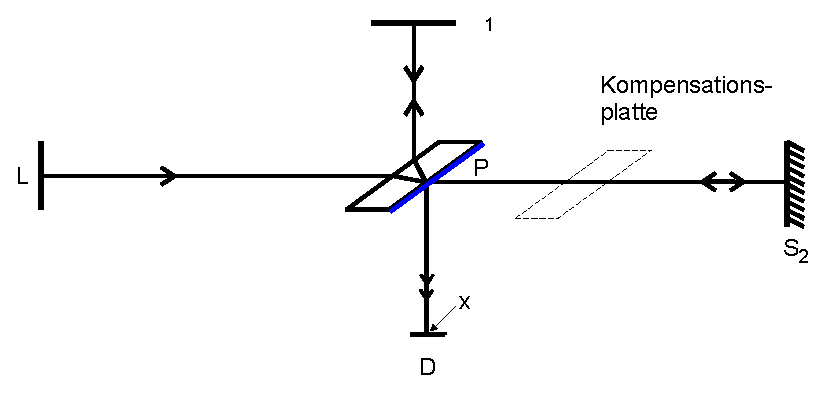
\includegraphics[height = 6cm]{michelson.pdf}
    \caption{Prinzipieller Aufbau des Michelson-interferometers \cite{ap401}.}
    \label{fig:michelson}
\end{figure}
Um Interferenzerscheinungen zu beobachten, muss das Licht kohärent sein, d.h. der Weglängenunterschied muss kleiner als die Kohärenzlänge $l$ sein. 
Aus diesem Grund wird er Abstand beider Spiegel gleich gewählt und eine Kompensationsplatte zwischen P und $\symup{S_2}$ eingebaut, sodass der längere 
Weg des Lichtstrahls zu $\symup{S_1}$ kompensiert wird. Wenn nun einer der Spiegel um $\symup{\Delta}d$ verschoben wird, ändert sich die detektierte 
Intensität. Es gilt
\begin{equation*}
    \symup{\Delta}d = z \cdot \frac{\lambda}{2} \; ,
\end{equation*}
wobei $z$ die Anzahl der Helligkeitsmaxima beschreibt.

\subsection{Bestimmung des Brechungsindex}
In \autoref{fig:mod} ist eine Modifizierung des Michelson-Interferometers dargestellt, bei der ein Medium der Länge $b$ in einen Strahlengang 
gesetzt wird.
\begin{figure}
    \centering
    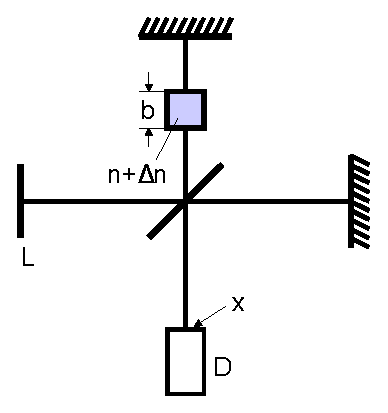
\includegraphics[height = 6cm]{modbrech.pdf}
    \caption{Modifizierung des Michelson-interferometers zur Messung des Brechungsindex \cite{ap401}.}
    \label{fig:mod}
\end{figure}
Der optische Wegunterschied ergibt sich damit zu 
\begin{equation*}
    b\symup{\Delta} = \frac{z\cdot\lambda}{2} \; . 
\end{equation*}
Durch die Dispersionsbeziehung ergibt sich für den Brechungsindex $n$
\begin{equation*}
    n = \sqrt{1+f\left(\lambda\right)\text{N}} \; .
\end{equation*}
Mit der idealen Gasgleichung, der Loschmidtschen Zahl $N_{\symup{L}}$ sowie einigen Umformungen kann der Brechungsindex über
\begin{equation*}
    n\left(p_0, T_0\right) = 1 + \frac{z\lambda T p_0}{2bT_0\left(p-p'\right)}
\end{equation*}
berechnet werden. 